%%%%%%%%%%%%%%%%%%%%%%%%%%%%%%%%%%%%%%%%%
% Stylish Curriculum Vitae
% LaTeX Template
% Version 1.1 (September 10, 2021)
%
% This template originates from:
% https://www.LaTeXTemplates.com
%
% Authors:
% Stefano (https://www.kindoblue.nl)
% Vel (vel@LaTeXTemplates.com)
%
% License:
% CC BY-NC-SA 4.0 (https://creativecommons.org/licenses/by-nc-sa/4.0/)
%
%%%%%%%%%%%%%%%%%%%%%%%%%%%%%%%%%%%%%%%%%
% !TEX program = xelatex
\documentclass[a4paper, oneside, final, 12pt]{scrartcl} % Paper options using the scrartcl class

\usepackage{fontspec} % for other font
\usepackage{xeCJK} % for chinese font
\usepackage{hyperref} % for hyper web link
\usepackage{multirow} % for tabular table in learning progress
\usepackage{graphicx} % for image insersion
\usepackage[export]{adjustbox} % for image frame
\usepackage{setspace}
\usepackage{array}
% Define typographic struts, as suggested by Claudio Beccari
%   in an article in TeX and TUG News, Vol. 2, 1993.
\usepackage{mathptmx}
\usepackage{scrlayer-scrpage} % Provides headers and footers configuration
\usepackage{titlesec} % Allows creating custom \section's
\usepackage{marvosym} % Allows the use of symbols
\usepackage{tabularx,colortbl} % Advanced table configurations
% \usepackage{ebgaramond} % Use the EB Garamond font
\usepackage{microtype} % To enable letterspacing
\usepackage{pdfpages} % for showing pdf
\usepackage{pdflscape}
\usepackage{enumitem}
\usepackage{subcaption}
\usepackage{listings}   % highlight the python code
\usepackage{xcolor}
\usepackage{multirow}
\usepackage{cite} %Imports biblatex package
\usepackage[ruled,linesnumbered]{algorithm2e}
\newcommand\mycommfont[1]{\normalsize\ttfamily\textcolor{blue}{#1}}
\SetCommentSty{mycommfont}
% \usepackage[backend=bibtex,bibencoding=ascii,style=authoryear,sorting=none]{bibtex}
% \addbibresource{reference.bib}
% setup the margin
\usepackage[top=1cm, bottom=1cm, right=2cm, left=2cm]{geometry}

% set the style of listing code
\definecolor{codegreen}{rgb}{0,0.6,0}
\definecolor{codegray}{rgb}{0.5,0.5,0.5}
\definecolor{codepurple}{rgb}{0.58,0,0.82}
\definecolor{backcolour}{rgb}{0.95,0.95,0.92}

\lstdefinestyle{mystyle}{
    backgroundcolor=\color{backcolour},   
    commentstyle=\color{codegreen},
    keywordstyle=\color{magenta},
    numberstyle=\tiny\color{codegray},
    stringstyle=\color{codepurple},
    basicstyle=\ttfamily\footnotesize,
    breakatwhitespace=true,         
    breaklines=true,                 
    captionpos=b,                    
    keepspaces=true,                 
    numbers=left,                    
    numbersep=5pt,                  
    showspaces=false,                
    showstringspaces=false,
    showtabs=false,                  
    tabsize=2
}

\lstset{style=mystyle}

% set chinese and english font
\setmainfont{Times New Roman}
\setCJKmainfont[AutoFakeBold=true, AutoFakeSlant=true]{標楷體}

\titleformat{\section}{\Large\raggedright\bfseries}{}{0em}{}[\titlerule] % Section formatting
\titleformat{\subsection}{\large\raggedright\bfseries}{}{0em}{}
\titleformat{\subsubsection}{\normalsize\raggedright\bfseries}{}{0em}{}

% \pagestyle{scrheadings} % Print the headers and footers on all pages

% enable bold and slant chinese font
% \xeCJKsetup{AutoFakeBold=true, AutoFakeSlant=true}

% set the space at the front of paragraph
\setlength{\parindent}{2em}

% disable page number
\pagenumbering{gobble}

\newcommand{\gray}{\rowcolor[gray]{.90}} % Custom highlighting for the work experience and education sections
\newcommand{\Tstrut}{\rule{0pt}{2.6ex}}         % = `top' strut
\newcommand{\Bstrut}{\rule[-0.9ex]{0pt}{0pt}}   % = `bottom' strut
\newcommand{\Tstruth}{\rule{0pt}{4ex}}         % = `top' strut for header
\newcommand{\Bstruth}{\rule[-2.5ex]{0pt}{0pt}}   % = `bottom' strut for header

%----------------------------------------------------------------------------------------
%	FOOTER SECTION
%----------------------------------------------------------------------------------------

% \renewcommand{\headfont}{\normalfont\rmfamily\scshape} % Font settings for footer

% \cofoot{
% \fontsize{12.5}{17}\selectfont % Letter spacing and font size

% \textls[150]{123 Broadway {\large\textperiodcentered} City {\large\textperiodcentered} Country 12345}\\ % Your mailing address
% {\Large\Letter} \textls[150]{john@smith.com \ {\Large\Telefon} (000) 111-1111} % Your email address and phone number
% }

%----------------------------------------------------------------------------------------
\begin{document}

%----------------------------------------------------------------------------------------
%	HEADER SECTION
%----------------------------------------------------------------------------------------


\begin{center}
    {\fontsize{18}{30}\textbf{NYCU 2023 Autumn \\ Data Visulization HW9 Report}} \\
\end{center}

\begin{center}
  Bo-Han Chen (陳柏翰) \\
  Student ID:312551074 \\
  bhchen312551074.cs12@nycu.edu.tw
\end{center}

\section{Overview}

In this homework, I use several data visulization method to show the details of
Spotify Track Dataset. The dataset contains 114000 songs and 19 features.
Figure \ref{fig: overview} shows the overview of my visulization system.
I will introduce the details of each part in the following sections.

\begin{figure}[h]
  \centering
  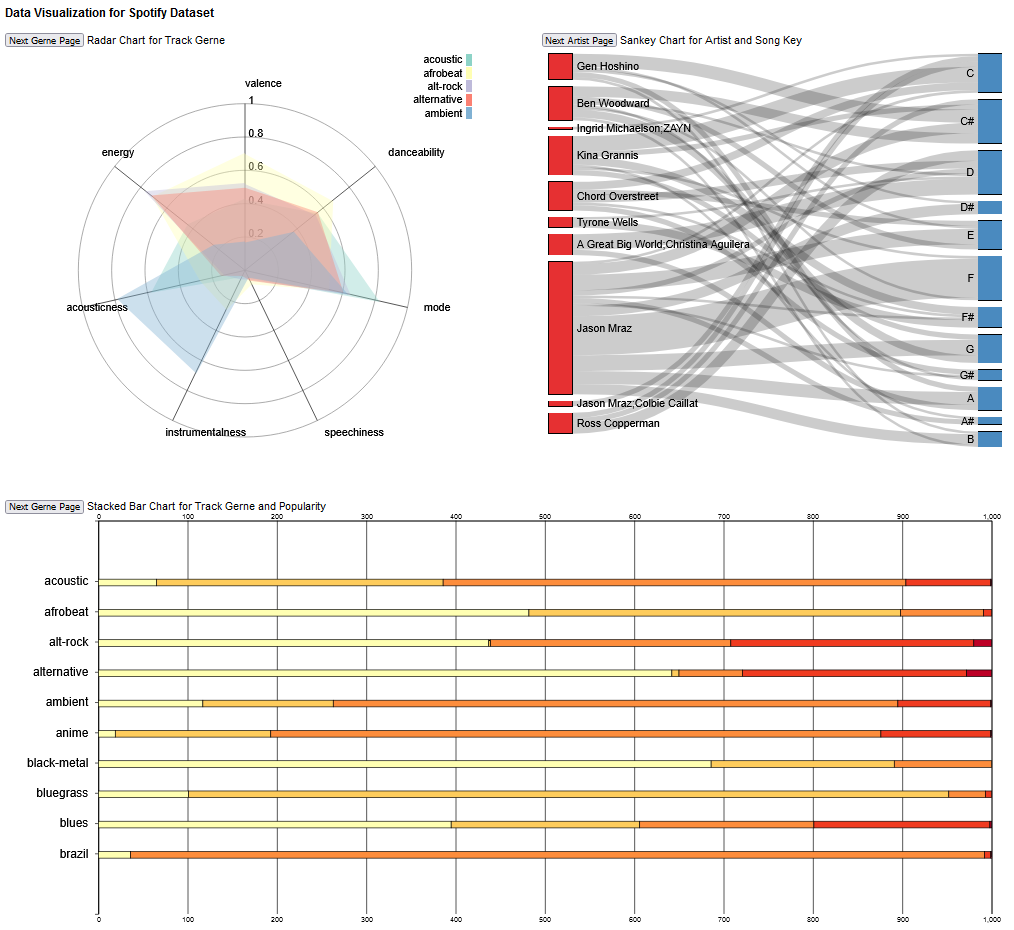
\includegraphics[width=0.8\textwidth]{Images/overview.png}
  \caption{Overview of my visulization system}
  \label{fig: overview}
\end{figure}

\section{Data Visulization}

\subsection{Radar Chart}

The first part of my visulization system is radar chart, which shows the
difference between each track gerne from the perspective of several features such as
acousticness, danceability, energy, instrumentalness, speechiness, valence and mode.
With the radar chart, we cannot only see the difference between each gerne, but
also discover the relationship between each feature.
For example, from the Figure \ref{fig: radar}, we can see that the difference between
classical and comedy music is very obvious, 
the former has higher acousticness and instrumentalness,
while the latter has higher speechiness and energy.
In the same figure, we can also discover the relationship between mode and valence,
when the mode is tend to be major, 
the corresponding valence is also tend to be happier (higher).

\begin{figure}[h]
  \centering
  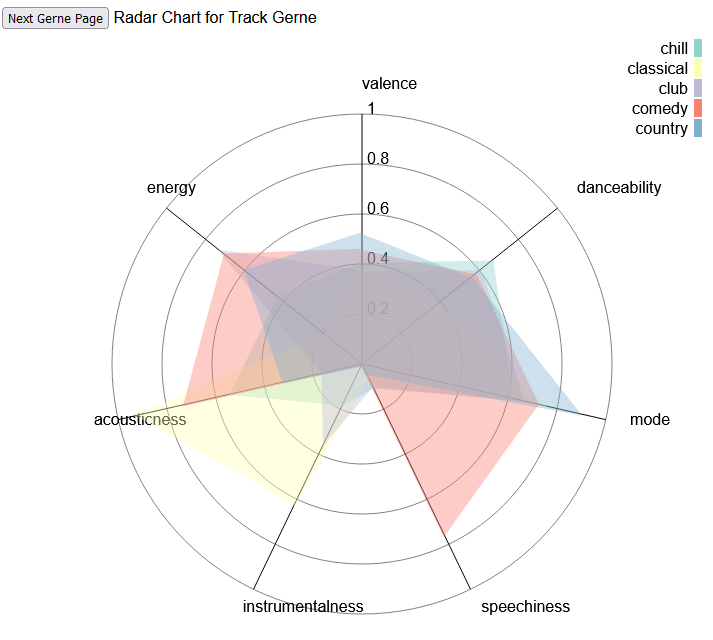
\includegraphics[width=0.8\textwidth]{Images/radar.png}
  \caption{Radar Chart}
  \label{fig: radar}
\end{figure}

\subsection{Sankey Diagram}

The second part of my visulization system is sankey diagram, which shows the relationship
between the artists and the track key.
With sankey diagram, we can see the distributon of track key of each artists,
which implies the their music style.
From Figure \ref{fig: sankey}, we can see that most of the selected artists prefer to
use C, C\# and D as their track key.
From the aspect of artist, the track key of Ross Copperman
is mainly C, C\# and D, which implies the music style of Ross Copperman is tend to be
happy and bright.

\begin{figure}[h]
  \centering
  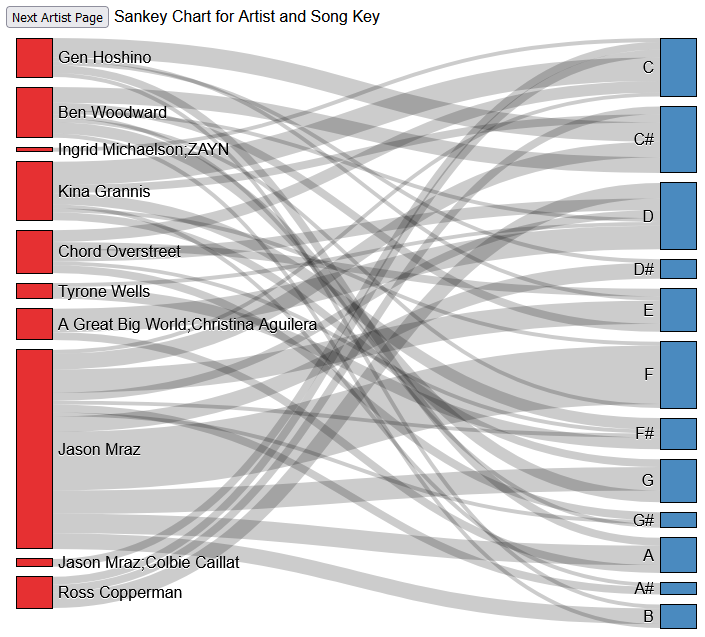
\includegraphics[width=0.8\textwidth]{Images/sankey.png}
  \caption{Sankey Diagram}
  \label{fig: sankey}
\end{figure}

\subsection{Stacked Bar Chart}

The third part is the stacked bar chart, which shows the distribution of popularity
of each gerne. In this dataset, each gerne has 1000 tracks, so we can easily to compare
the popularoty of each gerne.
From Figure \ref{fig: stacked}, we can see that the gerne with more high-popularity tracks
is K-Pop, which is well-known in worldwide.
For gerne such as Italian, while it has some 80-100\% popularity tracks,
the ratio of 0-20\% popularity tracks is obviously high, which implies Italian gerne
might have some hit song, but most of the them are not quite popular in Spotify.

\begin{figure}[ht]
  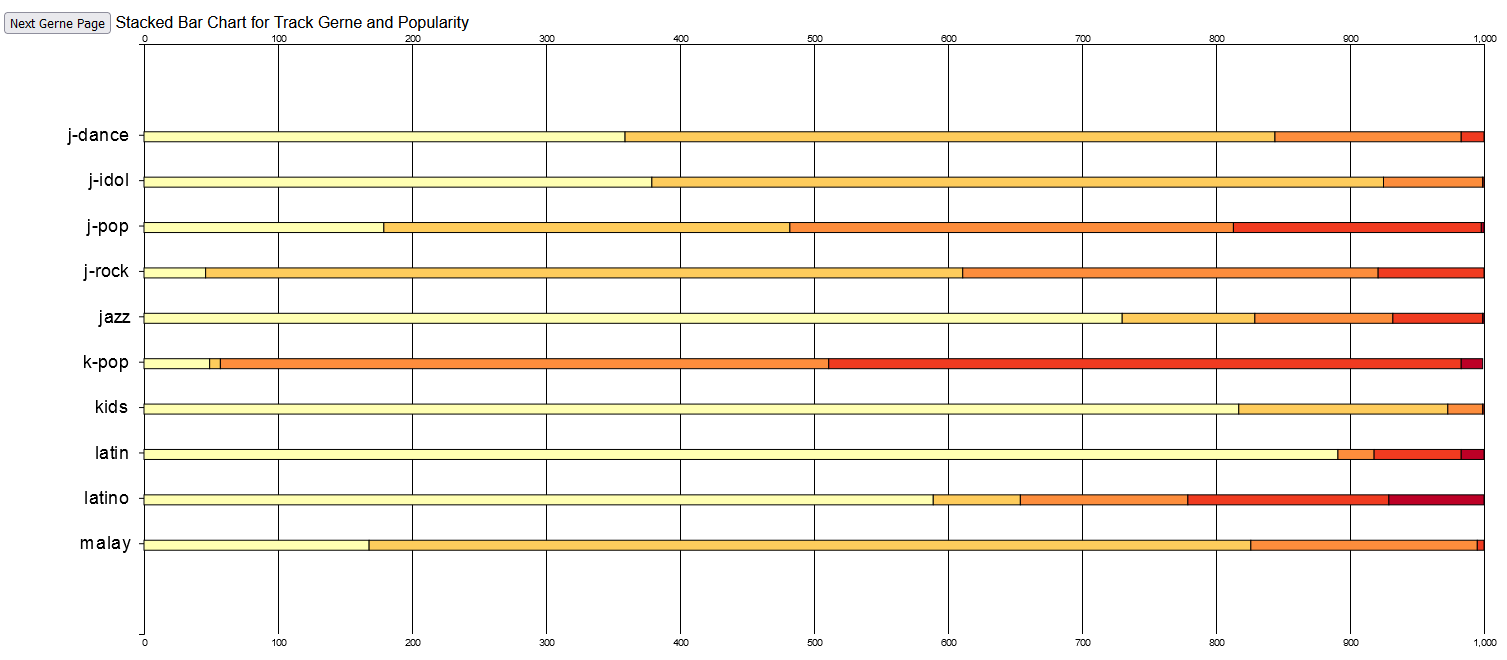
\includegraphics[width=\textwidth]{Images/stacked_bar_chart.png}
  \caption{Stacked Bar Chart}
  \label{fig: stacked}
\end{figure}

\section{Conclusion}

From the visulization system introduced above, 
we can see the trend and difference between each gerne or artists in the Spotify Track Dataset,
and discover the relationship between detailed feature.

\bibliographystyle{unsrt} % We choose the "plain" reference style
\bibliography{reference} % Entries are in the "references.bib" file

\end{document}